% coding:utf-8

%----------------------------------------
%FOSAPHY, a LaTeX-Code for a summary of basic physics
%Copyright (C) 2013, Daniel Winz, Ervin Mazlagic

%This program is free software; you can redistribute it and/or
%modify it under the terms of the GNU General Public License
%as published by the Free Software Foundation; either version 2
%of the License, or (at your option) any later version.

%This program is distributed in the hope that it will be useful,
%but WITHOUT ANY WARRANTY; without even the implied warranty of
%MERCHANTABILITY or FITNESS FOR A PARTICULAR PURPOSE.  See the
%GNU General Public License for more details.
%----------------------------------------

\section{Einfache harmonische Schwingung}
Die einfache harmonische Schwingung beschreibt ein System, welches 
nur zwei Energiespeicher hat. Ein klassisches Beispiel
ist die an einer Feder befestigte Masse. Um ein 
schwingfähiges System zu erhalten, muss es Wirkungen geben welche
entgegengesetzt sind. Im Beispiel aus Abbildung 
\ref{fig:einfache-harmonische} gibt es die zwei Kräfte $\vec{F}_k$ und
$\vec{F}_m$ die entgegengesetzt sind.

\begin{figure}[h!]
	\centering
	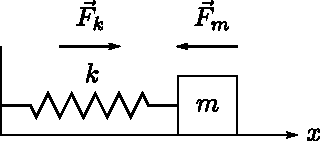
\includegraphics[scale=0.75]{../fig/einfache-harmonische.pdf}
	\caption{Einfach harmonisches Schwinungssystem}
	\label{fig:einfache-harmonische}
\end{figure}

\begin{figure}[h!]
	\centering
	\begin{tikzpicture}[domain=0:4]
		\draw[->] (-0.1,0) -- (5,0) node[below] {$t$};
		\draw[->] (0,-2.5) -- (0,2.5) node[left] {$x$};

		\draw[color=red, samples=200] plot[id=x] 
			function{0.5*cos(2*x)};
		\draw[color=blue, samples=200] plot[id=v] 
			function{-2*0.5*sin(2*x)};
		\draw[color=green, samples=200] plot[id=a] 
			function{-2*2*0.5*cos(2*x)};

		\draw[red] (4,2) node[right] 
			{$x(t) = A \sin(\omega t + \varphi)$};
		\draw[blue] (4,1.5) node[right] 
			{$\dot{x}(t) = -\omega A \cos(\omega t + \varphi)$};
		\draw[green] (4,1) node[right]
			{$\ddot{x}(t) = -\omega^2 A \sin(\omega t + \varphi)$};

		\draw[] (0.1,0.5) -- (-0.1,0.5) node[left] {$A$};
		\draw[] (0.1,1) -- (-0.1,1) node[left] {$\omega A$};
		\draw[]	(0.1,2) -- (-0.1,2) node[left] {$\omega^2 A$};
	\end{tikzpicture}
	\caption{Plot der einfachen harmonischen Schwingung}
\end{figure}

\subsection{Differentialgleichung}
Der Zusammenhang aus Abbildung \ref{fig:einfache-harmonische} stellt 
direkt die allgemeine Form des Systems als Differentialgleichung auf zu
\[ \boxed{\vec{F}_\Sigma  
	= \vec{F}_m + \vec{F}_k
	= m \cdot \ddot{x} + k \cdot x
	= 0
} \]

Der Weg, die Geschwindigkeit und die Beschleunigung lassen sich analog
zur linearen Bewegung durch Ableitungen und Integrale voneinander herleiten.
\[ \boxed{ \begin{array}{c c l}
	x(t) & = & 
		A \cdot \cos(\omega \cdot t + \varphi) \\
	\dot{x}(t) & = & 
		-\omega A \cdot \sin(\omega \cdot t + \varphi) \\
	\ddot{x}(t) & = & 
		-\omega^2 A \cdot \cos(\omega \cdot t + \varphi)
\end{array}}\]

Die Amplitude $A$ und die Phasenverschiebung $\varphi$ bietet die  
Parametierung der Bewegung an. Diese sind bei der einfachen harmonischen 
und ungedämpften Schwinung stets konstant. Die Kreisfrequenz $\omega$ 
beschreibt die Dynamik des Systems, also die \textit{Schnelligkeit}.
Diese kann aber auch mittels der Frequenz $f$ oder der Periodendauer $T$
ausgedrückt werden. 
\[ \boxed{ 
	\omega = 2 \pi f = 2 \pi \frac{1}{T}
	\quad \Rightarrow \quad
	f = \frac{\omega}{2 \pi} 
	\quad \Rightarrow \quad 
	T = \frac{2 \pi}{\omega} = \frac{1}{f} \\
} \]
Bei einfachen harmonischen Systemen wie in Abbildung 
\ref{fig:einfache-harmonische} ist die Dynamik definiert durch das
Verhältnis von Feder und Masse.
\[ \boxed{
	\omega = \sqrt{\frac{k}{m}}
}\]

